%% bare_conf.tex
%% V1.3
%% 2007/01/11
%% by Michael Shell
%% See:
%% http://www.michaelshell.org/
%% for current contact information.
%%
%% This is a skeleton file demonstrating the use of IEEEtran.cls
%% (requires IEEEtran.cls version 1.7 or later) with an IEEE conference paper.
%%
%% Support sites:
%% http://www.michaelshell.org/tex/ieeetran/
%% http://www.ctan.org/tex-archive/macros/latex/contrib/IEEEtran/
%% and
%% http://www.ieee.org/

%%*************************************************************************
%% Legal Notice:
%% This code is offered as-is without any warranty either expressed or
%% implied; without even the implied warranty of MERCHANTABILITY or
%% FITNESS FOR A PARTICULAR PURPOSE! 
%% User assumes all risk.
%% In no event shall IEEE or any contributor to this code be liable for
%% any damages or losses, including, but not limited to, incidental,
%% consequential, or any other damages, resulting from the use or misuse
%% of any information contained here.
%%
%% All comments are the opinions of their respective authors and are not
%% necessarily endorsed by the IEEE.
%%
%% This work is distributed under the LaTeX Project Public License (LPPL)
%% ( http://www.latex-project.org/ ) version 1.3, and may be freely used,
%% distributed and modified. A copy of the LPPL, version 1.3, is included
%% in the base LaTeX documentation of all distributions of LaTeX released
%% 2003/12/01 or later.
%% Retain all contribution notices and credits.
%% ** Modified files should be clearly indicated as such, including  **
%% ** renaming them and changing author support contact information. **
%%
%% File list of work: IEEEtran.cls, IEEEtran_HOWTO.pdf, bare_adv.tex,
%%                    bare_conf.tex, bare_jrnl.tex, bare_jrnl_compsoc.tex
%%*************************************************************************

% *** Authors should verify (and, if needed, correct) their LaTeX system  ***
% *** with the testflow diagnostic prior to trusting their LaTeX platform ***
% *** with production work. IEEE's font choices can trigger bugs that do  ***
% *** not appear when using other class files.                            ***
% The testflow support page is at:
% http://www.michaelshell.org/tex/testflow/



% Note that the a4paper option is mainly intended so that authors in
% countries using A4 can easily print to A4 and see how their papers will
% look in print - the typesetting of the document will not typically be
% affected with changes in paper size (but the bottom and side margins will).
% Use the testflow package mentioned above to verify correct handling of
% both paper sizes by the user's LaTeX system.
%
% Also note that the "draftcls" or "draftclsnofoot", not "draft", option
% should be used if it is desired that the figures are to be displayed in
% draft mode.
%
\documentclass[conference]{IEEEtran}
% Add the compsoc option for Computer Society conferences.
%
% If IEEEtran.cls has not been installed into the LaTeX system files,
% manually specify the path to it like:
% \documentclass[conference]{../sty/IEEEtran}





% Some very useful LaTeX packages include:
% (uncomment the ones you want to load)


% *** MISC UTILITY PACKAGES ***
%
%\usepackage{ifpdf}
% Heiko Oberdiek's ifpdf.sty is very useful if you need conditional
% compilation based on whether the output is pdf or dvi.
% usage:
% \ifpdf
%   % pdf code
% \else
%   % dvi code
% \fi
% The latest version of ifpdf.sty can be obtained from:
% http://www.ctan.org/tex-archive/macros/latex/contrib/oberdiek/
% Also, note that IEEEtran.cls V1.7 and later provides a builtin
% \ifCLASSINFOpdf conditional that works the same way.
% When switching from latex to pdflatex and vice-versa, the compiler may
% have to be run twice to clear warning/error messages.




% *** CITATION PACKAGES ***
%
%\usepackage{cite}
% cite.sty was written by Donald Arseneau
% V1.6 and later of IEEEtran pre-defines the format of the cite.sty package
% \cite{} output to follow that of IEEE. Loading the cite package will
% result in citation numbers being automatically sorted and properly
% "compressed/ranged". e.g., [1], [9], [2], [7], [5], [6] without using
% cite.sty will become [1], [2], [5]--[7], [9] using cite.sty. cite.sty's
% \cite will automatically add leading space, if needed. Use cite.sty's
% noadjust option (cite.sty V3.8 and later) if you want to turn this off.
% cite.sty is already installed on most LaTeX systems. Be sure and use
% version 4.0 (2003-05-27) and later if using hyperref.sty. cite.sty does
% not currently provide for hyperlinked citations.
% The latest version can be obtained at:
% http://www.ctan.org/tex-archive/macros/latex/contrib/cite/
% The documentation is contained in the cite.sty file itself.






% *** GRAPHICS RELATED PACKAGES ***
%
\ifCLASSINFOpdf
  \usepackage[pdftex]{graphicx}
  % declare the path(s) where your graphic files are
  % \graphicspath{{../pdf/}{../jpeg/}}
  % and their extensions so you won't have to specify these with
  % every instance of \includegraphics
  % \DeclareGraphicsExtensions{.pdf,.jpeg,.png}
\else
  % or other class option (dvipsone, dvipdf, if not using dvips). graphicx
  % will default to the driver specified in the system graphics.cfg if no
  % driver is specified.
  % \usepackage[dvips]{graphicx}
  % declare the path(s) where your graphic files are
  % \graphicspath{{../eps/}}
  % and their extensions so you won't have to specify these with
  % every instance of \includegraphics
  % \DeclareGraphicsExtensions{.eps}
\fi
% graphicx was written by David Carlisle and Sebastian Rahtz. It is
% required if you want graphics, photos, etc. graphicx.sty is already
% installed on most LaTeX systems. The latest version and documentation can
% be obtained at: 
% http://www.ctan.org/tex-archive/macros/latex/required/graphics/
% Another good source of documentation is "Using Imported Graphics in
% LaTeX2e" by Keith Reckdahl which can be found as epslatex.ps or
% epslatex.pdf at: http://www.ctan.org/tex-archive/info/
%
% latex, and pdflatex in dvi mode, support graphics in encapsulated
% postscript (.eps) format. pdflatex in pdf mode supports graphics
% in .pdf, .jpeg, .png and .mps (metapost) formats. Users should ensure
% that all non-photo figures use a vector format (.eps, .pdf, .mps) and
% not a bitmapped formats (.jpeg, .png). IEEE frowns on bitmapped formats
% which can result in "jaggedy"/blurry rendering of lines and letters as
% well as large increases in file sizes.
%
% You can find documentation about the pdfTeX application at:
% http://www.tug.org/applications/pdftex





% *** MATH PACKAGES ***
%
\usepackage[cmex10]{amsmath} %needed for align*
% A popular package from the American Mathematical Society that provides
% many useful and powerful commands for dealing with mathematics. If using
% it, be sure to load this package with the cmex10 option to ensure that
% only type 1 fonts will utilized at all point sizes. Without this option,
% it is possible that some math symbols, particularly those within
% footnotes, will be rendered in bitmap form which will result in a
% document that can not be IEEE Xplore compliant!
%
% Also, note that the amsmath package sets \interdisplaylinepenalty to 10000
% thus preventing page breaks from occurring within multiline equations. Use:
%\interdisplaylinepenalty=2500
% after loading amsmath to restore such page breaks as IEEEtran.cls normally
% does. amsmath.sty is already installed on most LaTeX systems. The latest
% version and documentation can be obtained at:
% http://www.ctan.org/tex-archive/macros/latex/required/amslatex/math/


% *** SPECIALIZED LIST PACKAGES ***
%
%\usepackage{algorithmic}
% algorithmic.sty was written by Peter Williams and Rogerio Brito.
% This package provides an algorithmic environment fo describing algorithms.
% You can use the algorithmic environment in-text or within a figure
% environment to provide for a floating algorithm. Do NOT use the algorithm
% floating environment provided by algorithm.sty (by the same authors) or
% algorithm2e.sty (by Christophe Fiorio) as IEEE does not use dedicated
% algorithm float types and packages that provide these will not provide
% correct IEEE style captions. The latest version and documentation of
% algorithmic.sty can be obtained at:
% http://www.ctan.org/tex-archive/macros/latex/contrib/algorithms/
% There is also a support site at:
% http://algorithms.berlios.de/index.html
% Also of interest may be the (relatively newer and more customizable)
% algorithmicx.sty package by Szasz Janos:
% http://www.ctan.org/tex-archive/macros/latex/contrib/algorithmicx/




% *** ALIGNMENT PACKAGES ***
%
%\usepackage{array}
% Frank Mittelbach's and David Carlisle's array.sty patches and improves
% the standard LaTeX2e array and tabular environments to provide better
% appearance and additional user controls. As the default LaTeX2e table
% generation code is lacking to the point of almost being broken with
% respect to the quality of the end results, all users are strongly
% advised to use an enhanced (at the very least that provided by array.sty)
% set of table tools. array.sty is already installed on most systems. The
% latest version and documentation can be obtained at:
% http://www.ctan.org/tex-archive/macros/latex/required/tools/


%\usepackage{mdwmath}
%\usepackage{mdwtab}
% Also highly recommended is Mark Wooding's extremely powerful MDW tools,
% especially mdwmath.sty and mdwtab.sty which are used to format equations
% and tables, respectively. The MDWtools set is already installed on most
% LaTeX systems. The lastest version and documentation is available at:
% http://www.ctan.org/tex-archive/macros/latex/contrib/mdwtools/


% IEEEtran contains the IEEEeqnarray family of commands that can be used to
% generate multiline equations as well as matrices, tables, etc., of high
% quality.


%\usepackage{eqparbox}
% Also of notable interest is Scott Pakin's eqparbox package for creating
% (automatically sized) equal width boxes - aka "natural width parboxes".
% Available at:
% http://www.ctan.org/tex-archive/macros/latex/contrib/eqparbox/





% *** SUBFIGURE PACKAGES ***
% \usepackage[tight,footnotesize]{subfigure}
% subfigure.sty was written by Steven Douglas Cochran. This package makes it
% easy to put subfigures in your figures. e.g., "Figure 1a and 1b". For IEEE
% work, it is a good idea to load it with the tight package option to reduce
% the amount of white space around the subfigures. subfigure.sty is already
% installed on most LaTeX systems. The latest version and documentation can
% be obtained at:
% http://www.ctan.org/tex-archive/obsolete/macros/latex/contrib/subfigure/
% subfigure.sty has been superceeded by subfig.sty.



% \usepackage[caption=false]{caption}
% \usepackage[font=footnotesize]{subfig}
% subfig.sty, also written by Steven Douglas Cochran, is the modern
% replacement for subfigure.sty. However, subfig.sty requires and
% automatically loads Axel Sommerfeldt's caption.sty which will override
% IEEEtran.cls handling of captions and this will result in nonIEEE style
% figure/table captions. To prevent this problem, be sure and preload
% caption.sty with its "caption=false" package option. This is will preserve
% IEEEtran.cls handing of captions. Version 1.3 (2005/06/28) and later 
% (recommended due to many improvements over 1.2) of subfig.sty supports
% the caption=false option directly:
% \usepackage[caption=false,font=footnotesize]{subfig}
%
% The latest version and documentation can be obtained at:
% http://www.ctan.org/tex-archive/macros/latex/contrib/subfig/
% The latest version and documentation of caption.sty can be obtained at:
% http://www.ctan.org/tex-archive/macros/latex/contrib/caption/




% *** FLOAT PACKAGES ***
%
%\usepackage{fixltx2e}
% fixltx2e, the successor to the earlier fix2col.sty, was written by
% Frank Mittelbach and David Carlisle. This package corrects a few problems
% in the LaTeX2e kernel, the most notable of which is that in current
% LaTeX2e releases, the ordering of single and double column floats is not
% guaranteed to be preserved. Thus, an unpatched LaTeX2e can allow a
% single column figure to be placed prior to an earlier double column
% figure. The latest version and documentation can be found at:
% http://www.ctan.org/tex-archive/macros/latex/base/



%\usepackage{stfloats}
% stfloats.sty was written by Sigitas Tolusis. This package gives LaTeX2e
% the ability to do double column floats at the bottom of the page as well
% as the top. (e.g., "\begin{figure*}[!b]" is not normally possible in
% LaTeX2e). It also provides a command:
%\fnbelowfloat
% to enable the placement of footnotes below bottom floats (the standard
% LaTeX2e kernel puts them above bottom floats). This is an invasive package
% which rewrites many portions of the LaTeX2e float routines. It may not work
% with other packages that modify the LaTeX2e float routines. The latest
% version and documentation can be obtained at:
% http://www.ctan.org/tex-archive/macros/latex/contrib/sttools/
% Documentation is contained in the stfloats.sty comments as well as in the
% presfull.pdf file. Do not use the stfloats baselinefloat ability as IEEE
% does not allow \baselineskip to stretch. Authors submitting work to the
% IEEE should note that IEEE rarely uses double column equations and
% that authors should try to avoid such use. Do not be tempted to use the
% cuted.sty or midfloat.sty packages (also by Sigitas Tolusis) as IEEE does
% not format its papers in such ways.





% *** PDF, URL AND HYPERLINK PACKAGES ***
%
%\usepackage{url}
% url.sty was written by Donald Arseneau. It provides better support for
% handling and breaking URLs. url.sty is already installed on most LaTeX
% systems. The latest version can be obtained at:
% http://www.ctan.org/tex-archive/macros/latex/contrib/misc/
% Read the url.sty source comments for usage information. Basically,
% \url{my_url_here}.


% *** Custom Packages ***
\usepackage[]{mcode}

% *** Custom Commands ***
\newcommand{\cphi}{c\phi}
\newcommand{\cth}{c\theta}
\newcommand{\cpsi}{c\psi}
\newcommand{\sphi}{s\phi}
\newcommand{\sth}{s\theta}
\newcommand{\spsi}{s\psi}
\newcommand{\E}{\mathbf{E}}
\newcommand{\e}{\mathbf{e}}


% *** Do not adjust lengths that control margins, column widths, etc. ***
% *** Do not use packages that alter fonts (such as pslatex).         ***
% There should be no need to do such things with IEEEtran.cls V1.6 and later.
% (Unless specifically asked to do so by the journal or conference you plan
% to submit to, of course. )


% correct bad hyphenation here
\hyphenation{op-tical net-works semi-conduc-tor}


\begin{document}
%
% paper title
% can use linebreaks \\ within to get better formatting as desired
\title{MIMO Sliding Control for Quadcopter}


% author names and affiliations
% use a multiple column layout for up to three different
% affiliations
\author{
\IEEEauthorblockN{Dennis Wai}
\IEEEauthorblockA{UC Berkeley Mechanical Engineering Department\\
Email: dwai213@gmail.com\\
SID: 2118 3965}}


% make the title area
\maketitle


\begin{abstract}
Based on Newton's principles, the dynamics model, both second and first order, for the quadcopter is derived. The quadcopter model is then used to design a sliding mode controller to achieve tracking on reference inputs. The sliding mode controller is designed through feedback linearization and thus stability of internal dynamics are investigated. A PD controller is also designed to serve as a baseline and benchmark for the SMC controller. Simulations for two reference inputs, a step and sinusoid, are presented to compare and contrast the SMC's performance.
\end{abstract}
% IEEEtran.cls defaults to using nonbold math in the Abstract.
% This preserves the distinction between vectors and scalars. However,
% if the conference you are submitting to favors bold math in the abstract,
% then you can use LaTeX's standard command \boldmath at the very start
% of the abstract to achieve this. Many IEEE journals/conferences frown on
% math in the abstract anyway.

% no keywords




% For peer review papers, you can put extra information on the cover
% page as needed:
% \ifCLASSOPTIONpeerreview
% \begin{center} \bfseries EDICS Category: 3-BBND \end{center}
% \fi
%
% For peerreview papers, this IEEEtran command inserts a page break and
% creates the second title. It will be ignored for other modes.
\IEEEpeerreviewmaketitle



\section{Introduction}
The quadcopter is a mobile platform that ranges from the size of a palm to the size of a laptop. The highly maneuverable platform opens up a new realm of exploratory and inspection possibilities. However, precise control is very desirable for full autonomous operations. This report will go over two control strategies for a general quadcopter model and their derivation in Section \ref{implementation}. Then in Section \ref{simulation}, the simulation setup will be presented while Section \ref{results} will compare the simulation results between the two control strategies. Notable results and summary will be provided in Section \ref{conclude}.

In the upcoming sections, the following nomenclature will be used:
\begin{table}[h]
\centering
\begin{tabular}{|l|l|}
\hline
\textbf{Symbol} & \textbf{Definition}                    \\ \hline
$m$             & Quadcopter Mass                        \\ \hline
$g$             & Acceleration due to gravity            \\ \hline
$l$             & Distance between quadcopter center of mass and a rotor \\ \hline
$I_j$           & Quadcopter rotational inertia in $j$ axis, $j \in \{ x,y,z\}$ \\ \hline
$x$,$y$,$z$     & Quadcopter $x$,$y$,$z$ coordinate in world frame \\ \hline
$\phi$, $\theta$, $\psi$ & Quadcopter body angle: roll, pitch, yaw  \\ \hline
$C_j$           & Translational drag coefficient in $j$ axis, $j \in \{ x,y,z\}$ \\ \hline
$C_j'$          & Rotational drag coefficient in $j$ axis, $j \in \{ \phi,\theta,\psi \}$  \\ \hline
$F_i$           & Thrust generated by rotor $i$, $i \in [ 1,4 ]$  \\ \hline
$\omega_i$      & Rotor Speed for rotor $i$, $i \in [ 1,4 ]$  \\ \hline
$M_i$           & Moment generated by rotor $i$, $i \in [ 1,4 ]$   \\ \hline
$K_f$           & Motor constant for force for all rotors  \\ \hline
$K_m$           & Motor constant for moments for all rotors  \\ \hline
$\E_j$          & World frame unit vector in the $j$ axis, $j \in \{ x,y,z\}$ \\ \hline
$\e_j$          & Body frame unit vector in the $j$ axis, $j \in \{ x,y,z\}$ \\ \hline
$u_i$           & Control inputs ($\omega_i$) for the PD controller  \\ \hline
$u_i'$          & Control inputs for the sliding controller  \\ \hline
$v_i$           & The $i$th state variable for the quadcopter system in first order\\ \hline
$s_i$           & The $i$th attractive surface for the sliding controller  \\ \hline
$v'$            & The synthetic control in feedback linearization  \\ \hline
$v_i'$          & The $i$th term in $v'$  \\ \hline
$\eta_i$       & The $i$th gain for the $i$th surface  \\ \hline
$c\phi$ and $s\phi$ & Shorthand for $\cos{(\phi)}$ and $\sin{(\phi)}$ \\ \hline
\end{tabular}
\end{table}

\section{Implementation} \label{implementation}
\subsection{Dynamics and Modeling}
Taking \cite{bib:model} as a reference, I employed Newtonian principles to arrive at the equation of motion for the quadcopter. First, I use the standard Yaw-Pitch-Roll parameterization for the quadcopter's rotation.
\begin{align*}
R_{WB} &= \begin{bmatrix}
 \cpsi & -\spsi   & 0\\ 
 \spsi & \cpsi  & 0\\ 
 0 & 0 & 1
\end{bmatrix}
\begin{bmatrix}
 \cth & 0   & \sth\\ 
 0 & 1  & 0\\ 
 -\sth & 0 & \cth
\end{bmatrix}
\begin{bmatrix}
 1 & 0   & 0\\ 
0 & \cphi  & \sphi\\ 
 0 & -\sphi & \cphi
\end{bmatrix} \\
R_{WB} &= 
\begin{bmatrix}
 \cth\cphi & \cpsi\sth\sphi - \cphi\spsi   & \sth\cphi\cpsi + \spsi\sphi\\ 
\cth\spsi & \sth\sphi\spsi + \cphi\cpsi  & \sth\cphi\spsi - \cpsi\sphi\\ 
 -\sth & \cth\sphi & \cth\cphi 
\end{bmatrix} \\
&= 
\begin{bmatrix}
\E_x \cdot \e_x & \E_x \cdot \e_y   & \E_x \cdot \e_z \\ 
\E_y \cdot \e_x & \E_y \cdot \e_y   & \E_y \cdot \e_z \\ 
\E_z \cdot \e_x & \E_z \cdot \e_y   & \E_z \cdot \e_z \\ 
\end{bmatrix}
\end{align*}
where $R_{WB}$ is the transformation that takes coordinates in the quadcopter body frame to the world frame.

The free body diagram and annotated diagram for the quadcopter is provided in Fig. \ref{fig:fbd} and Fig. \ref{fig:quadcopter}, respectively. 
\begin{figure}[!ht]
\centering
\includegraphics[width=2.5in]{images/fbd.png}
\caption{Free body diagram for a quadcopter. Note that drag forces are not pictured here for brevity and clarity, but it is understood that they all appear in their respective dimensions as a resistive force. The rotors are also numbered here.}
\label{fig:fbd}
\end{figure}

\begin{figure}[!ht]
\centering
\includegraphics[width=2.5in]{images/quadcopter.png}
\caption{Annotated diagram for the quadcopter with the body and world frame defined here as $O_W$ adn $O_B$, respectively.}
\label{fig:quadcopter}
\end{figure}

Starting from Newton's second law and summing forces in the three Cartesian direction, we arrive at the following equations:
\begin{align*}
m\mathbf{a} &= \sum F_i \e_z + \mathbf{F_{drag}} - mg \E_z \\
\\
m\ddot{x} &= \sum F_i \e_z \cdot \E_x - C_x\dot{x} \\
m\ddot{y} &= \sum F_i \e_z \cdot \E_y - C_y\dot{y} \\
m\ddot{z} &= \sum F_i \e_z \cdot \E_z - mg - C_z\dot{z} \\
\\ 
m\ddot{x} &= \sum F_i (\spsi\sphi + \cpsi\sth\cphi) - C_x\dot{x} \\
m\ddot{y} &= \sum F_i (\spsi\sth\cphi - \cpsi\sphi) - C_y\dot{y} \\
m\ddot{z} &= \sum F_i (\cth\cphi) - mg - C_z\dot{z}
\end{align*}
where the summation is $i = 1 \dots 4$ for the four rotors. It is assumed that each rotor's thrust are characterized identically and prescribed by $F_i = K_f\omega_i^2$. 

Starting from Newton's second law and summing moments in the three Cartesian direction, we arrive at the following equations:
\begin{align*}
I_x\ddot{\phi} \e_x &+ I_y\ddot{\theta} \e_y + I_z\ddot{\psi} \e_z = \sum\mathbf{M_j} + \mathbf{M_{drag}}\\
\\
I_x\ddot{\phi} &= l(F_3 - F_1 - C_x' \dot{\phi}) \\
I_y\ddot{\theta} &= l(F_4 - F_2 - C_y' \dot{\theta}) \\
I_z\ddot{\psi} &= M_1 - M_2 + M_3 - M_4 - C_z'\dot{\psi}
\end{align*}
where the summation is $j \in [x,y,z]$ for the moments generated by forces in the three axes. It is assumed that each rotor's reaction moment are characterized identically and prescribed by $M_i = K_m\omega_i^2$. 

For simulation and sliding control design purposes, I convert this to a series of first ordinary differential equations by prescribing the state variable $v$:
\begin{align*}
\mathbf{v} = \begin{bmatrix} x \\ \dot{x} \\ y \\ \dot{y} \\ z \\ \dot{z} \\ \phi \\ \dot{\phi} \\ \theta \\ \dot{\theta} \\ \psi \\ \dot{\psi} \end{bmatrix} =
\begin{bmatrix} v_1 \\ v_2 \\ v_3 \\ v_4 \\ v_5 \\ v_6 \\ v_7 \\ v_8 \\ v_9 \\ v_{10} \\ v_{11} \\ v_{12}\end{bmatrix}
\end{align*}
Taking the derivative, we arrive at the following first order system, which can be used for simulation as well as design.
\begin{align*}
\dot{\mathbf{v}} = \begin{bmatrix}
v_2 \\
\frac{1}{m}(\sum F_i (\spsi\sphi + \cpsi\sth\cphi) - C_xv_2) \\
v_4 \\
\frac{1}{m}(\sum F_i (\spsi\sth\cphi - \cpsi\sphi)  - C_yv_4)\\
v_6 \\
\frac{1}{m}(\sum F_i (\cth\cphi) - C_zv_6) - g \\
v_8 \\
l(F_3 - F_1 - C_\phi'v_8)\frac{1}{I_x} \\
v_{10} \\
l(F_4 - F_2 - C_\theta'v_{10})\frac{1}{I_y} \\
v_{12} \\
(M_1 - M_2 + M_3 - M_4 - lC_\psi'v_{12})\frac{1}{I_z}
\end{bmatrix}
\end{align*}

\subsection{PD Controller Design}
The PD control strategy is chosen in this report to serve as a reference to the sliding controller that will be discussed later. In the PD case, the control inputs are considered to be the four rotor speeds (i.e. $u_i = \omega_i, i \in [1,4]$). This is somewhat arbitrary because $u_i = F_i$ is also a suitable candidate for a control input. First, I define $K_* = (K_p^{(*)} +K_d^{(*)}\frac{d}{dt})$, or the PD gain used on the $*$ channel (e.g. $y$) error, $\widetilde{y} = y_d - y$. (Note that $\frac{d}{dt}$ is the differentiation operator.) The prescription for the controller is given by the expression below.
\begin{align*}
w_1 &= K_y\widetilde{y} + K_z\widetilde{z} - K_\phi\widetilde{\phi} + K_\psi\widetilde{\psi} \\
w_2 &= -K_x\widetilde{x} + K_z\widetilde{z} - K_\theta\widetilde{\theta} - K_\psi\widetilde{\psi} \\
w_3 &= -K_y\widetilde{y} + K_z\widetilde{z} + K_\phi\widetilde{\phi} + K_\psi\widetilde{\psi} \\
w_4 &= K_x\widetilde{x} + K_z\widetilde{z} + K_\theta\widetilde{\theta} - K_\psi\widetilde{\psi} \\
\end{align*}

The controller architecture is shown in Fig. \ref{fig:pd_controller}.
\begin{figure}[!ht]
\centering
\includegraphics[width=3.2in]{images/pd_controller.png}
\caption{Diagram of the PD control architecture}
\label{fig:pd_controller}
\end{figure}
One advantage of the PD controller is that it is model-agnostic and doesn't require any more knowledge of the system. We conclude our design of the PD controller.

\subsection{Sliding Controller Design}
Before we begin in a design of a sliding controller for this system, we first redefine our control inputs as demonstrated in \cite{bib:inputs} to simplify the controller design. We define the control inputs $u_i'$ (note the prime symbol) for this controller to be:
\begin{align*}
u_1' &= F_1+F_2+F_3+F_4 \\
u_2' &= F_3-F_1 \\
u_3' &= F_4-F_2 \\
u_4' &= F_1-F_2+F_3-F_4
\end{align*}
The individual rotor thrust can be determined by inverting the relationship between $u_i'$ and $F_i$. The inverse relationship is:
\begin{align*}
F_1 &= 0.25u_1' - 0.50u_2' + 0.25u_4' \\
F_2 &= 0.25u_1' - 0.50u_3' - 0.25u_4' \\
F_3 &= 0.25u_1' + 0.50u_2' + 0.25u_4' \\
F_4 &= 0.25u_1' + 0.50u_3' - 0.25u_4'
\end{align*}
Next, we also reorganize the terms in our first order system so that we can more easily recognize the underlying structure.
\begin{align*}
\dot{\mathbf{v}} &= f(x) + g(x)u' \\
f(x) &= \begin{bmatrix}
v_2 \\
-\frac{C_x}{m}v_2 \\
v_4 \\
-\frac{C_y}{m}v_4 \\
v_6 \\
-\frac{C_z}{m}v_6 - g \\
v_8 \\
-\frac{lC_\phi'}{I_x}v_8 \\
v_{10} \\
-\frac{lC_\theta'}{I_y}v_{10} \\
v_{12} \\
-\frac{lC_\psi'}{I_z}v_{12} \\
\end{bmatrix} \ \ \ \ u' = \begin{bmatrix}
u_1' \\ u_2' \\ u_3' \\ u_4' \end{bmatrix}
\end{align*}
\begin{align*}
g(x) = \begin{bmatrix}
0 & 0 & 0 & 0 \\
\frac{1}{m}(\spsi\sphi + \cpsi\sth\cphi) & 0 & 0 & 0 \\
0 & 0 & 0 & 0 \\
\frac{1}{m}(\spsi\sth\cphi - \cpsi\sphi)  & 0 & 0 & 0 \\
0 & 0 & 0 & 0 \\
\frac{1}{m} (\cth\cphi)  & 0 & 0 & 0 \\
0 & 0 & 0 & 0 \\
0 & \frac{l}{I_x} & 0 & 0 \\
0 & 0 & 0 & 0 \\
0 & 0 &  \frac{l}{I_y} & 0\\
0 & 0 & 0 & 0 \\
0 & 0 & 0 & \frac{K_f}{K_mI_z}
\end{bmatrix}
\end{align*}
Taking inspiration from the general MIMO sliding mode control section in \cite{bib:hedrick}, we chose four outputs ($z,\phi,\theta,\psi$) and performed input/output feedback linearization. The linearized equations with a total of $4 \times 2$ relative degrees are:
\begin{align*}
y_1 &= z = v_5 \\
\dot{y_1} &= v_6 \\
\ddot{y_1} &= -\frac{C_z}{m}v_6 - g + \frac{1}{m}(\cth\cphi) u_1' \\
\\
y_2 &= \phi = v_7 \\
\dot{y_2} &= v_8 \\
\ddot{y_2} &= -\frac{lC_\phi'}{I_x}v_8 + \frac{l}{I_x} u_2' \\
\\
y_3 &= \theta = v_{9} \\
\dot{y_3} &= v_{10} \\
\ddot{y_3} &= -\frac{lC_\theta'}{I_y}v_{10} + \frac{l}{I_y} u_3' \\
\\
y_4 &= \psi = v_{11} \\
\dot{y_4} &= v_{12} \\
\ddot{y_4} &= -\frac{lC_\psi'}{I_z}v_{12} + \frac{K_f}{K_mI_z} u_4' 
\end{align*}
Following \cite{bib:hedrick}, the prescription for the control inputs $u'$ is:
\begin{align*}
u' = J^{-1}(v'-l_1)
\end{align*}
where
\begin{align*}
J &= \begin{bmatrix}
 \frac{(\cth\cphi) }{m} & 0 & 0 & 0\\ 
 0 & \frac{l}{I_x} & 0 & 0\\ 
 0 & 0 & \frac{l}{I_y}  & 0 \\ 
 0 & 0 & 0 & \frac{K_f}{K_mI_z} 
\end{bmatrix} \\
l_1 &= \begin{bmatrix}
-\frac{C_z}{m}v_6 - g - \ddot{y_{1d}} + \beta_{11}(\dot{y_1} - \dot{y_{1d}})\\
-\frac{lC_\phi'}{I_x}v_8 - \ddot{y_{2d}} + \beta_{21}(\dot{y_2} - \dot{y_{2d}})  \\
-\frac{lC_\theta'}{I_y}v_{10} - \ddot{y_{3d}} + \beta_{31}(\dot{y_3} - \dot{y_{3d}})   \\
-\frac{lC_\psi'}{I_z}v_{12} - \ddot{y_{4d}} + \beta_{41}(\dot{y_4} - \dot{y_{4d}})   \\
\end{bmatrix}
\end{align*}
and
\begin{align*}
v' &= \begin{bmatrix}
v_1' \\
v_2' \\
v_3' \\
v_4'
\end{bmatrix} \ \ \ \
v_i' = -\eta_i\frac{s_i}{\Phi_i} \\
s_i &=  \dot{y_{i}} - \dot{y_{id}} + \beta_{i1}(y_i - y_{id})
\end{align*}
where $i \in [1 \dots 4]$.
\subsubsection{Stability}
The prescribed $s_i$ are the sliding surfaces the system states are attracted to. The attraction is guaranteed because the condition $s\dot{s} < -\eta_i\frac{s^2}{\Phi_i}$ is satisfied. We show this for the second surface:
\begin{align*}
\dot{s_2} &=  \ddot{y_{2}} - \ddot{y_{2d}} + \beta_{21}(\dot{y_2} - \dot{y_{2d}}) \\
&= -\frac{lC_\phi'}{I_x}v_8 + \frac{l}{I_x} u_2' - \ddot{y_{2d}} + \beta_{21}(\dot{y_2} - \dot{y_{2d}})
\end{align*}
Taking the second row, $u_2'$ from $u'$:
\begin{align*}
u_2' &= \frac{I_x}{l} (v_2' + \frac{lC_\phi'}{I_x}v_8 + \ddot{y_{2d}} - \beta_{21}(\dot{y_2} - \dot{y_{2d}}) )
\end{align*}
We can substitute into the original expression to find that:
\begin{align*}
\dot{s_2} &=  v_2' = -\eta_2\frac{s_2}{\Phi_2}  \\
&\longrightarrow s\dot{s} = -\eta_2\frac{s_2^2}{\Phi_2} < 0  \\
\end{align*}
Therefore, the surface is attractive and the dynamics at $s=0$ will be achieved. In our prescription for $s_i$, the system will achieve perfect tracking with the desired signal at the $i$th channel. In our example here, the system's $\phi(t)$ will track perfectly the reference signal, $\phi_d(t)$.


\subsubsection{Internal Dynamics}
The dimensionality of the internal dynamics manifold is 4 because $n-r = 4$, where $n = 12$. The internal states are ($\phi,\theta$) and are defined by the diffeomorphism below:
\begin{align*}
\begin{bmatrix}
z_1 \\ \vdots \\ z_r \\ \xi_1 \\ \vdots \\ \xi_{n-r}
\end{bmatrix} = 
T
\begin{bmatrix}
v_1 \\ \vdots \\ \vdots \\ \vdots \\ v_{12}
\end{bmatrix}
\end{align*}
where $T$ is the $12\times12$ identity matrix with the first 4 rows taken out and then appended to the bottom of the same identity matrix (i.e the transformation T takes the first four state equations from the $\dot{\mathbf{v}}$ and puts them at the bottom).

Checking the zero dynamics, we find that the internal dynamics are governed by ordinary differential equations of the form:
\begin{align*}
\dot{h} = -\frac{C_j}{m}h
\end{align*}
which is a trivially stable system since $\frac{C_j}{m} > 0$. Therefore, the internal states are stable.

\subsubsection{Addendum}
An astute student would observe that if there was an error in the internal states (i.e. $x$), then the prescribed controller would be unable to do anything. In fact, error in the channels concerning the internal states do not appear in $u'$. For that reason, it is necessary to tie error in these channels with appropriate corrective action in channels that the controller controls. For example, if there is error in the $x$ channel, the quadcopter should prescribe a $\theta_d(t)$ trajectory that can correct this error. The underlying trick here is to acknowledge that pitching ($\theta \neq 0$) will cause the quadcopter to move along the x-axis. Inspired by \cite{bib:topology} and the aforementioned, the sliding control controller topology is shown in Fig. \ref{fig:smc_controller}. The important addition is the reference generator would translate desirable $x_d(t)$ trajectories into $\theta_d(t)$ trajectories that can be tracked by our controller. For this implementation,
\begin{align*}
\theta_d(t) = K_{\theta_d}\widetilde{x}
\end{align*}
where $K_{\theta_d}$ are tunable parameters. A similar prescription will also apply for $\phi_d(t)$ trajectories.

\begin{figure}[!ht]
\centering
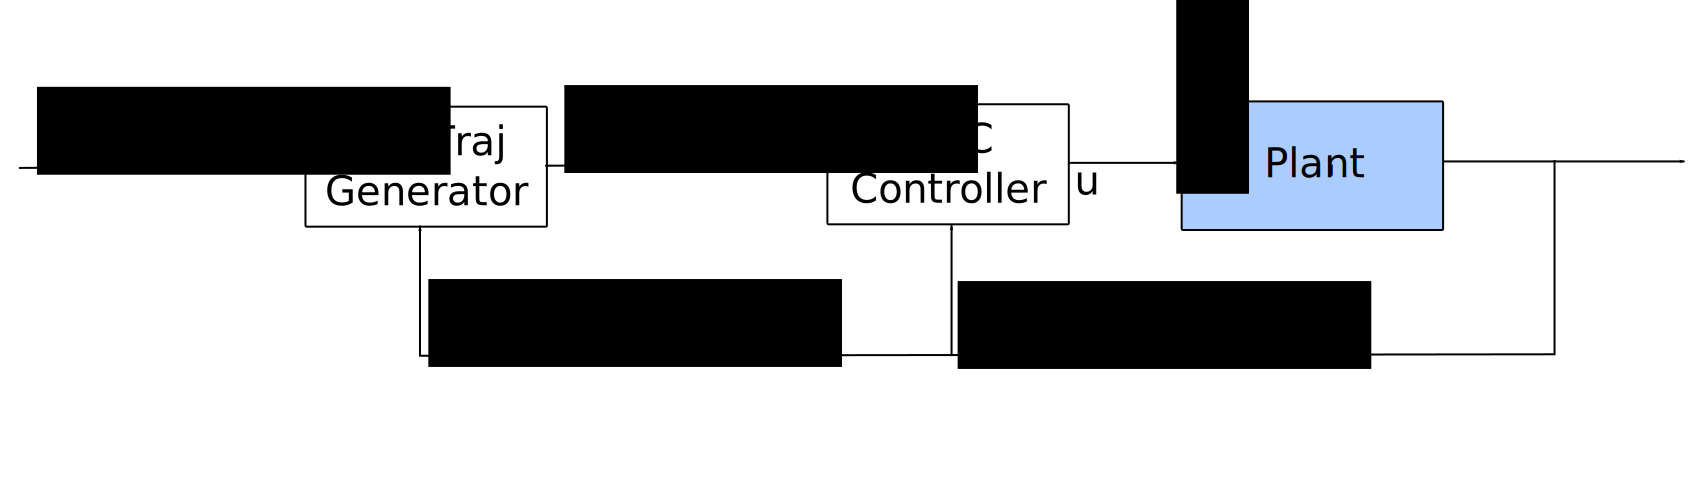
\includegraphics[width=3.2in]{images/smc_controller.png}
\caption{Diagram of the sliding controller architecture with the addition of a reference generator block that translates $x_d(t)$ and $y_d(t)$ trajectories into $\theta_d(t)$ and $\phi_d(t)$, respectively.}
\label{fig:smc_controller}
\end{figure}

\section{Simulation Set Up} \label{simulation}
For all simulations, Table. \ref{tbl:sim_params} lists the parameter values, which were loosely based off of an off-the-shelf quadcopter.
\begin{table}
\centering
\begin{tabular}{|l|l|}
\hline
\textbf{Parameter} & \textbf{Initialization}                    \\ \hline
$m$             & .5                        \\ \hline
$g$             & 9.81 \\ \hline
$l$             & .25 \\ \hline
$I_j$           & [0.0042 0.0042 0.0312] \\ \hline
$x$,$y$,$z$     & [0 0 .2] \\ \hline
$\phi$, $\theta$, $\psi$ & [0 0 0] \\ \hline
$C_j$           & 0 \\ \hline
$C_j'$          & 0  \\ \hline
$K_f$           & 100  \\ \hline
$K_m$           & 1  \\ \hline
\end{tabular}
\caption{Table of simulation parameters, in SI units unless otherwise specified}
\label{tbl:sim_params}
\end{table}

\subsection{PD Controller}
The PD controller is implemented in \verb|Simulink| and is shown in Fig. \ref{fig:pd_mdl}
\begin{figure}[!ht]
\centering
\includegraphics[width=3.2in]{images/pd_mdl.png}
\caption{Screen capture of the simulation for the PD controller and quadcopter}
\label{fig:pd_mdl}
\end{figure}

\subsection{Sliding Control} 
The SMC controller is implemented in \verb|Simulink| and is shown in Fig. \ref{fig:smc_mdl}.
\begin{figure}[!ht]
\centering
\includegraphics[width=3.2in]{images/smc_mdl.png}
\caption{Screen capture of the simulation for the sliding controller and quadcopter. Note the extra feedback path to the reference subsystem.}
\label{fig:smc_mdl}
\end{figure}

The reference generator was also implemented in \verb|Simulink| and is shown in Fig. \ref{fig:smc_ref_mdl}.
\begin{figure}[!ht]
\centering
\includegraphics[width=3.2in]{images/smc_ref_mdl.png}
\caption{The content of the inner reference subsystem. Note that the body angle desired trajectories are filtered Cartesian coordinate trajectories.}
\label{fig:smc_ref_mdl}
\end{figure}

\section{Results and Analysis} \label{results}
Because both the PD controller and the sliding controller are tunable, it is hard to rigorously compare the two control techniques. Both controllers were tuned to approximately the same performance for a given step input in the $x$ channel with a .1 amplitude. Subsequently, both controllers were then subjected to a sinusoidal reference signal (i.e. $x_d(t) = .1\sin{(t)}$) in the $x$ channel to assess the performance.
\subsection{PD Controller}
\subsubsection{Step Reference}
Two plots of the controller performance (state tracking (Fig. \ref{fig:pd_1}) and control input (Fig. \ref{fig:pd_2}) ) when given a step reference input is provided here.
\begin{figure}[!ht]
\centering
\includegraphics[width=3.2in]{../pd_1.png}
\caption{Plot of the Cartesian coordinates vs time for the PD controller. The black dashed line is the reference step input that the controller achieves tracking.}
\label{fig:pd_1}
\end{figure}
\begin{figure}[!ht]
\centering
\includegraphics[width=3.2in]{../pd_2.png}
\caption{Plot for the quadcopter rotor thrusts. Note the sinusoidal transient behavior}
\label{fig:pd_2}
\end{figure}
\subsubsection{Sinusoidal Reference}
Two plots of the controller performance (state tracking (Fig. \ref{fig:pd_5})  and error (Fig. \ref{fig:pd_7}) ) when given a sinusoidal reference input is provided here.
\begin{figure}[!ht]
\centering
\includegraphics[width=3.2in]{../pd_5.png}
\caption{Plot of the the quadcopter's Cartesian states when given a sinusoidal reference to track}
\label{fig:pd_5}
\end{figure}
\begin{figure}[!ht]
\centering
\includegraphics[width=3.2in]{../pd_7.png}
\caption{When given a sinusoidal reference, the PD controller cannot achieve perfect tracking as demonstrated by this plot of error vs time.}
\label{fig:pd_7}
\end{figure}

\subsection{Sliding Control}
\subsubsection{Step Reference}
Two plots of the controller performance (state tracking (Fig. \ref{fig:smc_1})  and control input (Fig. \ref{fig:smc_2}) ) when given a step reference input is provided here.
\begin{figure}[!ht]
\centering
\includegraphics[width=3.2in]{../smc_1.png}
\caption{Plot of the Cartesian coordinates vs time for the SMC controller. The black dashed line is the reference step input that the controller achieves tracking.}
\label{fig:smc_1}
\end{figure}
\begin{figure}[!ht]
\centering
\includegraphics[width=3.2in]{../smc_2.png}
\caption{Plot for the quadcopter rotor thrusts. Note the absence of any sinusoidal transient behavior}
\label{fig:smc_2}
\end{figure}
\subsubsection{Sinusoidal Reference}
Two plots of the controller performance (state tracking (Fig. \ref{fig:smc_5})  and error (Fig. \ref{fig:smc_7}) ) when given a sinusoidal reference input is provided here.
\begin{figure}[!ht]
\centering
\includegraphics[width=3.2in]{../smc_5.png}
\caption{Plot of the the quadcopter's Cartesian states when given a sinusoidal reference to track}
\label{fig:smc_5}
\end{figure}
\begin{figure}[!ht]
\centering
\includegraphics[width=3.2in]{../smc_7.png}
\caption{After several more rounds of tuning, the SMC controller achieves almost perfect tracking of the reference sinusoidal signal.}
\label{fig:smc_7}
\end{figure}

\subsubsection{Discussion}
From the above plots, both the PD and SMC controller boast similar performance to track a reference step input. (Fig. \ref{fig:pd_1} and Fig. \ref{fig:smc_1}) One noticeable difference is the control used by each controller. The PD controller prescribes a control (Fig. \ref{fig:pd_2}) that has transient sinusoidal behavior, which can make it harder to implement for low bandwidth systems. In contrast, the SMC controller prescribes a much smoother control (Fig. \ref{fig:smc_2}) and should be more implementable on physical systems.
\begin{figure}[!ht]
\centering
\includegraphics[width=3.2in]{../smc_best.png}
\caption{When given a sinusoidal reference, the SMC controller cannot achieve perfect tracking either. However, the magnitude of error compared to the PD controller is much smaller}
\label{fig:smc_best}
\end{figure}
Another improvement the SMC controller provides is better sinusoidal reference tracking. This difference is qualitatively observed between Fig. \ref{fig:pd_5} and Fig. \ref{fig:smc_5} where the SMC tracking performance is more in phase with the reference signal whereas the PD controller lags significantly behind the reference signal. Quantitatively, Fig. \ref{fig:pd_7} and Fig. \ref{fig:smc_7} highlights this contrast because the error for the SMC controller is less than that of the PD controller. However, Fig. \ref{fig:smc_best} shows that with proper tuning, the SMC controller can achieve good performance, even for sinusoidal reference inputs.

\section{Conclusion} \label{conclude}
Using basic Newton's principles, the dynamics model for a typical quadcopter was derived and transformed for a 12-dimensional first order system. SMC controller design involved input/output feedback linearization on the system. Although the dimensionality of the relative degree was less than that of the entire system, the internal dynamics were shown to be stable. Both PD and SMC control technique were applied to the system and achieved good tracking performance for a step reference input. Although both controllers showed less-than-perfect tracking performance for a sinusoidal reference, the SMC controller performed slightly better by 1) prescribing a smooth control input and 2) having less residual error. However, with proper tuning, the SMC controller can achieve almost perfect tracking performance. 



% trigger a \newpage just before the given reference
% number - used to balance the columns on the last page
% adjust value as needed - may need to be readjusted if
% the document is modified later
%\IEEEtriggeratref{8}
% The "triggered" command can be changed if desired:
%\IEEEtriggercmd{\enlargethispage{-5in}}

% references section

% can use a bibliography generated by BibTeX as a .bbl file
% BibTeX documentation can be easily obtained at:
% http://www.ctan.org/tex-archive/biblio/bibtex/contrib/doc/
% The IEEEtran BibTeX style support page is at:
% http://www.michaelshell.org/tex/ieeetran/bibtex/
%\bibliographystyle{IEEEtran}
% argument is your BibTeX string definitions and bibliography database(s)
%\bibliography{IEEEabrv,../bib/paper}
%
% <OR> manually copy in the resultant .bbl file
% set second argument of \begin to the number of references
% (used to reserve space for the reference number labels box)
\begin{thebibliography}{1}

\bibitem{bib:model}
Nemati, Alireza, and Manish Kumar. \emph{Modeling and control of a single axis tilting quadcopter.} American Control Conference (ACC), 2014. IEEE, 2014.

\bibitem{bib:topology}
Sumantri, Bambang, et al. \emph{Robust tracking control of a quad-Rotor helicopter utilizing sliding mode control with a nonlinear sliding surface.} Journal of System Design and Dynamics 7.2 (2013): 226-241.

\bibitem{bib:inputs}
Zhang, X. B., and Y. M. Zhang. \emph{Fault tolerant control for quad-rotor UAV by employing Lyapunov-based adaptive control approach.} AIAA Guidance, Navigation, and Control Conference. 2010.

\bibitem{bib:adapt}
Tony, Chau T., and William Mackunisy. \emph{Robust attitude tracking control of a quadrotor helicopter in the presence of uncertainty.} CDC. 2012.

\bibitem{bib:hedrick}
Hedrick, J., and Girard, A. (n.d.). Control of Nonlinear Dynamic Systems: Theory and Applications. 2010


\end{thebibliography}



% that's all folks
\end{document}



% An example of a floating figure using the graphicx package.
% Note that \label must occur AFTER (or within) \caption.
% For figures, \caption should occur after the \includegraphics.
% Note that IEEEtran v1.7 and later has special internal code that
% is designed to preserve the operation of \label within \caption
% even when the captionsoff option is in effect. However, because
% of issues like this, it may be the safest practice to put all your
% \label just after \caption rather than within \caption{}.
%
% Reminder: the "draftcls" or "draftclsnofoot", not "draft", class
% option should be used if it is desired that the figures are to be
% displayed while in draft mode.
%
%\begin{figure}[!t]
%\centering
%\includegraphics[width=2.5in]{myfigure}
% where an .eps filename suffix will be assumed under latex, 
% and a .pdf suffix will be assumed for pdflatex; or what has been declared
% via \DeclareGraphicsExtensions.
%\caption{Simulation Results}
%\label{fig_sim}
%\end{figure}

% Note that IEEE typically puts floats only at the top, even when this
% results in a large percentage of a column being occupied by floats.


% An example of a double column floating figure using two subfigures.
% (The subfig.sty package must be loaded for this to work.)
% The subfigure \label commands are set within each subfloat command, the
% \label for the overall figure must come after \caption.
% \hfil must be used as a separator to get equal spacing.
% The subfigure.sty package works much the same way, except \subfigure is
% used instead of \subfloat.
%
%\begin{figure*}[!t]
%\centerline{\subfloat[Case I]\includegraphics[width=2.5in]{subfigcase1}%
%\label{fig_first_case}}
%\hfil
%\subfloat[Case II]{\includegraphics[width=2.5in]{subfigcase2}%
%\label{fig_second_case}}}
%\caption{Simulation results}
%\label{fig_sim}
%\end{figure*}
%
% Note that often IEEE papers with subfigures do not employ subfigure
% captions (using the optional argument to \subfloat), but instead will
% reference/describe all of them (a), (b), etc., within the main caption.


% An example of a floating table. Note that, for IEEE style tables, the 
% \caption command should come BEFORE the table. Table text will default to
% \footnotesize as IEEE normally uses this smaller font for tables.
% The \label must come after \caption as always.
%
%\begin{table}[!t]
%% increase table row spacing, adjust to taste
%\renewcommand{\arraystretch}{1.3}
% if using array.sty, it might be a good idea to tweak the value of
% \extrarowheight as needed to properly center the text within the cells
%\caption{An Example of a Table}
%\label{table_example}
%\centering
%% Some packages, such as MDW tools, offer better commands for making tables
%% than the plain LaTeX2e tabular which is used here.
%\begin{tabular}{|c||c|}
%\hline
%One & Two\\
%\hline
%Three & Four\\
%\hline
%\end{tabular}
%\end{table}


% Note that IEEE does not put floats in the very first column - or typically
% anywhere on the first page for that matter. Also, in-text middle ("here")
% positioning is not used. Most IEEE journals/conferences use top floats
% exclusively. Note that, LaTeX2e, unlike IEEE journals/conferences, places
% footnotes above bottom floats. This can be corrected via the \fnbelowfloat
% command of the stfloats package.

